% !TeX spellcheck = de_DE
% !TeX encoding = UTF-8
% Vorlage Studien- und Diplomarbeiten, Bachelor- Masterarbeiten
%
% author: FG EMSP TU Berlin, Dipl.-Ing. Alexander Vorwerk
%
% last updated: 11.01.2011, by FG EMSP TU Berlin, Dipl.-Ing. Dennis lerch

% PREAMBLE, for use with pdfTex
% before documentclass
% disable pdfoutput to be able to include eps graphics and use packages like pstricks
% conversion dvi2ps and ps2pdf needed afterwards, pdftex specials like hyperref are still possible
%\pdfoutput=0                            % dvi output - use with pdfcprot (character protruding)

% \RequirePackage{fix-cm}                       % error correction for standard fonts

%% define CLASS
\documentclass[11pt, a4paper, parskip=half*, bibliography=totoc, cleardoublepage=empty, final,numbers=noenddot]{scrbook}                       % begin every chapter one left page
% \documentclass[11pt, a4paper, parskip=half*, bibliography=totoc, cleardoublepage=empty, final,
% numbers=noenddot]{scrreprt}                    % ongoing pages, no page break after chapter

%% misc
% !TEX root = thesis.tex

%% \usepackage{cmbright}                          % serifenlose computer modern fonts

% \usepackage{fontenc}                       % T1 fonts für gute pdf-Ausgabe
% \usepackage[utf8]{inputenc}                    % wegen deutschen Umlauten
\usepackage[automark]{scrlayer-scrpage}                % Koma Headers

% \usepackage[english]{babel}

\usepackage{nag}                               % warn user on outdated packages
\usepackage[linktocpage, hidelinks]{hyperref}  % links in pdf, thumbnails
\usepackage{soul}                              % emphasizing text, underlining
\usepackage[onehalfspacing]{setspace}          % 1.5, change line spaces by \singlespacing \doublespacing

%% tables
\usepackage{multicol}                          % multiple columns in tables
\usepackage{multirow}                          % multiple rows in tables
\usepackage[
  margin=10pt,
  labelfont=bf,
  figurewithin=chapter,
  tablewithin=chapter
]{caption} % table headers
\usepackage{hhline}                            % horizontal lines
\usepackage{longtable}                         % pagebreak tables
\usepackage{booktabs}                          % bold table lines, e.g. \toprule
\usepackage{tabularx}                          % neue Tabular-Umgebung

%% math, symbols
\usepackage{amsmath}                           % AMS Math like brackets, integrals...
\usepackage{amssymb}                           % AMS-Symbols v2.0
\usepackage{fixmath}                           % big greek letters italic in math mode
\usepackage{array}                             % matrices
\usepackage[per-mode=symbol]{siunitx}                           % includes nicefrac, nicer fracs for one line, SI-Units
\DeclareSIUnit{\bits}{bits}
\usepackage[integrals]{wasysym}                % for integrals like \oiint


\usepackage{microtype}                         % character protruding, font expansion - instead of pdfcprot
\usepackage{graphicx}                          % include graphics
\usepackage{wrapfig}                           % graphics in text
\usepackage{floatflt}                          % graphics/tables in text
\usepackage{rotating}                          % rotating elements

\usepackage[svgnames]{xcolor}                  % colors for listings
\usepackage{psfrag}                            % Text in .eps Grafiken ersetzen
\usepackage{float}
\usepackage[european]{circuitikz}
\usepackage{pgfplots}
 \pgfplotsset{compat=1.5}
\renewcommand{\rmdefault}{pplx}
\usepackage{eulervm}                           % math font



\usepackage{lipsum} % blind text

% code
\usepackage[
  cachedir=out/_minted-\jobname,
  outputdir=out/,
  chapter
]{minted}
\usemintedstyle{paraiso-light}
\AtBeginDocument{\DeclareCaptionSubType{listing}}
\renewcommand{\listingscaption}{Code Example}
\renewcommand{\listoflistingscaption}{List of Code Examples}

\usepackage{subcaption}  % subcaptions

\usepackage[noabbrev]{cleveref} % references
\crefname{sublisting}{code example}{code examples}
\Crefname{sublisting}{Code Example}{Code Examples}
\crefname{listing}{code example}{code examples}

\usepackage[
    acronym,
    style=longheader,
    % indexonlyfirst,
    nopostdot
    ]{glossaries-extra}
\renewcommand{\glossaryentrynumbers}[1]{\textcolor{blue}{#1}}
\setabbreviationstyle[acronym]{long-short} % first occurence long, rest short
\renewcommand*{\acrshort}[1][]{\glsxtrshort[noindex,#1]} % acrshort -> no index


\usepackage{bytefield}

\newcommand{\xor}{\ensuremath \veebar}

\usepackage{nicefrac}

\usetikzlibrary{external}
\tikzexternalize[prefix=tikz_out/]

\makeatletter
\DeclareRobustCommand{\skippedwords}[1][1ex]{%
  \setlength{\units@wide}{\bf@bitwidth * \bits@wide}%
  \setlength{\units@high}{1pt * \ratio{\units@wide}{9.0pt}}%
  \setlength{\units@tall}{#1 + \units@high}%
  \edef\num@wide{\strip@pt\units@wide}%
  \edef\num@tall{\strip@pt\units@tall}%
  \edef\num@high{\strip@pt\units@high}%
  \begin{tikzpicture}
    \draw (\linewidth,0) -- (0,0.5) -- (0,0);
    \draw (0,0.7) -- (\linewidth,0.2) -- (\linewidth,0.7);
  \end{tikzpicture}
  \ifcounting@words
    \inc@bytefield@height{\unitlength * \real{\num@tall}}%
    \global\counting@wordsfalse
  \fi}
  \makeatother

% \usepackage[datesep=., style=ddmmyyyy]{datetime2}
\newcommand{\leadingzero}[1]{\ifnum #1<10 0\the#1\else\the#1\fi}
\renewcommand{\today}{\leadingzero{\day}.\leadingzero{\month}.\the\year}


\usepackage[
    backend=biber,
    style=numeric,
  ]{biblatex}

 \addbibresource{bib.bib}

% \usepackage[all]{nowidow}
\usepackage[bottom]{footmisc}
\usepackage{csquotes}
\usepackage{etoolbox}
\usepackage{framed}

\newenvironment{multipagecode}{\captionsetup{type=listing}\vspace{1cm}}{}

\makeatletter
\newcommand*{\textoverline}[1]{$\overline{\hbox{#1}}\m@th$}
\makeatother

% twosided figure https://tex.stackexchange.com/a/23865/104727

% This class already provide the functionality of both
\usepackage[strict]{changepage}
\usepackage{adjustbox}
\usepackage{afterpage}
\usepackage{placeins}

\setcounter{totalnumber}{1}
\setcounter{topnumber}{1}
\setcounter{bottomnumber}{1}
\renewcommand{\topfraction}{.99}
\renewcommand{\bottomfraction}{.99}
\renewcommand{\textfraction}{.01}

\makeatletter
\newcommand*{\twopagepicture}[4]{%
    \checkoddpage
    \ifoddpage
        \expandafter\@firstofone
    \else
        \expandafter\afterpage
    \fi
    {\afterpage{%
    \begin{figure}[t]
        \makebox[\textwidth][l]{%
        \if #1p\relax
            \let\mywidth\paperwidth
            \hskip-\dimexpr1in+\hoffset+\evensidemargin\relax
            \hspace*{.05\mywidth}
            \adjustbox{trim=0 0 {.5\width} 0,clip}{\includegraphics[width=1.8\mywidth]{#2}}%
        \else
            \let\mywidth\paperwidth
            \hskip-\dimexpr1in+\hoffset+\evensidemargin\relax
            \hspace*{.1\mywidth}
            \adjustbox{trim=0 0 {.5\width} 0,clip}{\includegraphics[width=1.65\mywidth]{#2}}%
        \fi
        }
        \caption{#3}%
        \label{#4}%
    \end{figure}%
    \begin{figure}[t]
        \makebox[\textwidth][l]{%
        \if #1p%
            \let\mywidth\paperwidth
            \hskip-\dimexpr1in+\hoffset+\oddsidemargin\relax
            \hspace*{.05\mywidth}
            \adjustbox{trim={.5\width} 0 0 0,clip}{\includegraphics[width=1.8\mywidth]{#2}}%
        \else
            \let\mywidth\paperwidth
            \hskip-\dimexpr1in+\hoffset+\oddsidemargin\relax
            \hspace*{.1\mywidth}
            \adjustbox{trim={.5\width} 0 0 0,clip}{\includegraphics[width=1.65\mywidth]{#2}}%
        \fi
        }
    \end{figure}%
    }}%
}
\makeatother

\newcommand{\TODO}[1]{\begin{framed}%
  {\textcolor{red}{\Large TODO: #1}}%
\end{framed}%
}

% has to be at the end for some weird reason (https://tex.stackexchange.com/a/450540/104727)
\usepackage{fontspec}


\makeatletter
\usepackage{pdfpages}
\usetikzlibrary{external}
\tikzexternalize[prefix=figures/,shell escape=-enable-write18,optimize command away=\includepdf]

\graphicspath{{figures/}{logos/}{diagrams/}{plots/}}
% \makeatletter
% \def\input@path{{bytefields/}}
% \makeatother

%\ctikzset{voltage=german}

\makeatother
%% layout
\usepackage[top=2.5cm,left=3.5cm,right=2.5cm,bottom=3cm]{geometry}

%%%%%%%%%%%%%%%%%%%%%%%%%%%%%%%%%%%%%%%%%%%%%%%%%%%%
% document definitions, do not change
% Allgemeine Schalter - Änderung von Standardeinstellungen
\frenchspacing                                       % keine längeren Leerzeichen nach Satzende/Abkürzungen mit Punkt
\setlength{\parindent}{0pt}                          % kein Einzug bei neuem Absatz
\setlength{\parskip}{1.5ex plus0.5ex minus 0.5ex}    % Abstand zwischen 2 Absätzen

% verwende das paket setspace statt baselinestretch, Vorteil: Abstände in Fußzeilen und
% listenumgebungen etc. bleiben erhalten
\tolerance 1414
\hbadness 1414
\emergencystretch 1.5em
\hfuzz 0.3pt
\widowpenalty=10000
\vfuzz \hfuzz
\raggedbottom
\brokenpenalty=10000                                 % Trennung bei Seitenumbruch

\setlength{\headheight}{1cm}                         % Höhe der Kopfzeile
\addtolength{\footnotesep}{2pt}                      % abstand der Fußnote zur Trennlinie

% Setze Überschriftentiefe
\setcounter{secnumdepth}{3}                          % Nummerierung der Kapitel
\setcounter{figure}{4}                               % Bilder
\setcounter{tocdepth}{3}                             % Gliederungsebene für Inhaltsverzeichnis
\pagestyle{plain}
\clearscrheadings
\setheadsepline{.0pt}
% Einstellungen für Kopf- und Fußzeilen
\pagestyle{scrheadings}                              % nutze scrheader
\clearscrheadings                                    % lösche alle vorhandenen header

\setheadsepline{.05pt}                               % trennlinie oben
\setfootsepline{.05pt}                               % trennlinie unten

\automark[section]{chapter}   % links chapter, rechts section


\newcommand*{\Title}{Design and Implementation of a Model CPU with Basic Logic Chips and related Development Environment for Educational Purposes}
\newcommand*{\Author}{Niklas Schelten}
\newcommand*{\Date}{\today}
\title{\Title}
\author{\Author}
\date{\Date}

% variere nach ein-/zweiseitig
\makeatletter
\if@twoside                     % bei zweiseitig
  \lehead{\leftmark}            % setze Kapitel linke Seite oben
  \rohead{\rightmark}           % setze Abschnitt rechte Seite oben
  \lefoot{\pagemark}            % Seitennummer unten links
  \rofoot{\pagemark}            % Seitennummer unten rechts
  \lofoot{\Author}              % Name des Verfassers nur linke Seite
\else                           % einseitig
  \ihead{\leftmark}             % setze linke kopfzeile
  \ohead{\rightmark}            % setze rechte kopfzeile
  \ofoot{\pagemark}             % seitennummer unten rechts
  \ifoot{\Author}               % Name des Verfassers unten links
\fi
\makeatother

% !TEX root = ../thesis.tex
\makeglossaries
\newacronym{EDiC}{EDiC}{Educational Digital Computer}
\newacronym{RISC}{RISC}{Reduced Instruction Set Computer}
\newacronym{CISC}{CISC}{Complex Instruction Set Computer}
\newacronym{ALU}{ALU}{Arithmetic Logic Unit}
\newacronym{EEPROM}{EEPROM}{Electrically Erasable Programmable Read-Only Memory}
\newacronym{MAR}{MAR}{Memory Address Register}
\newacronym{RDMA}{RDMA}{Remote Direct Memory Access}
\newacronym{RoCEv2}{RoCEv2}{Remote Direct Memory Access over Converged Ethernet v2}
\newacronym{FPGA}{FPGA}{Field Programmable Gate Array}
\newacronym{ASIC}{ASIC}{Application-Specific Integrated Circuit}
\newacronym{UDP}{UDP}{User Datagram Protocol}
\newacronym{TCP}{TCP}{Transmission Control Protocol}
\newacronym{AXI}{AXI}{Advanced eXtensible Interface}
\newacronym{CPU}{CPU}{Central Processing Unit}
\newacronym{SIFT}{SIFT}{Scale-Invariant Feature Transform}
\newacronym{PCB}{PCB}{Printed Circuit Board}
\newacronym{DMA}{DMA}{Direct Memory Access}
\newacronym{RAM}{RAM}{Random-Access Memory}
\newacronym{SRAM}{SRAM}{Static Random-Access Memory}
\newacronym{IB}{IB}{InfiniBand}
\newacronym{IP}{IP}{Internet Protocol}
\newacronym{DSP}{DSP}{Digital Signal Processor}
\newacronym{BRAM}{BRAM}{Block RAM}
\newacronym{EPROM}{EPROM}{Erasable Programmable Read-Only Memory}
\newacronym{CLB}{CLB}{Configurable Logic Block}
\newacronym{LUT}{LUT}{Lookup Table}
\newacronym{MUX}{MUX}{Multiplexer}
\newacronym{MTU}{MTU}{Maximum Transmission Unit}
\newacronym{PSN}{PSN}{Package Sequence Number}
\newacronym{CM}{CM}{Connection Management}
\newacronym{RC}{RC}{Reliable Connection}
\newacronym{UD}{UD}{Unreliable Datagram}
\newacronym{ICRC}{ICRC}{Invariant Cycling Redundancy Check}
\newacronym{CRC}{CRC}{Cycling Redundancy Check}
\newacronym{IANA}{IANA}{Internet Assigned Number Authority}
\newacronym{TTL}{TTL}{Time To Live}
\newacronym{QP}{QP}{Queue Pair}
\newacronym{BTH}{BTH}{Base Transport Header}
\newacronym{DETH}{DETH}{Datagram Extended Transport Header}
\newacronym{MAD}{MAD}{Common Management Datagram}
\newacronym{RNR}{RNR}{Receiver Not Ready}
\newacronym{ARI}{ARI}{Additional Reject Information}
\newacronym{MSB}{MSB}{Most Significant Bit}
\newacronym{LSB}{LSB}{Least Significant Bit}
\newacronym{LRH}{LRH}{Local Routing Header}
\newacronym{GRH}{GRH}{Global Routing Header}
\newacronym{AETH}{AETH}{ACK Extended Transport Header}
\newacronym{RETH}{RETH}{RDMA Extended Transport Header}
\newacronym{NAK}{NAK}{Not Acknowledge}
\newacronym{MAC}{MAC}{Media Access Control}
\newacronym{DDR}{DDR}{Double Data Rate}
\newacronym{FIFO}{FIFO}{First In First Out Storage}
\newacronym{VHDL}{VHDL}{VHSIC (Very High Speed Integrated Circuit) Hardware Description Language}
\newacronym{VHSIC}{VHSIC}{Very High Speed Integrated Circuit}
\newacronym{HDL}{HDL}{Hardware Description Language}
\newacronym{LFSR}{LFSR}{Linear Feedback Shift Register}
\newacronym{DUT}{DUT}{Device Under Testing}
\newacronym{ALM}{ALM}{Adaptive Logic Module}
\newacronym{LAB}{LAB}{Logic Array Block}
\newacronym{MLAB}{MLAB}{Memory Logic Array Block}
\newacronym{OS}{OS}{Operating System}
\newacronym{TUB}{TUB}{Technical University Berlin}
\newacronym{IC}{IC}{Integrated Circuit}
\newacronym{LED}{LED}{Light-Emitting Diode}
\newacronym{PC}{PC}{Program Counter}
\newacronym{SP}{SP}{Stack Pointer}
\newacronym{NOP}{NOP}{No Operation}
\newacronym{CSON}{CSON}{CoffeeScript-Object-Notation}
\newacronym{JSON}{JSON}{JavaScript Object Notation}
\newacronym{PRNG}{PRNG}{Pseudo Random Number Generator}
\newacronym{UART}{UART}{Universal Asynchronous Receiver-Transmitter}
\newacronym{IDE}{IDE}{Integrated Development Environment}
\newacronym{ISA}{ISA}{Instruction Set Architecture}
\newacronym{EDIF}{EDIF}{Electronic Design Interchange Format}

%%%%%%%%%%%%%%% THESIS START %%%%%%%%%%%%%%
\begin{document}

% !TEX root = ../thesis.tex
\begin{titlepage}
\begin{centering}
	% Header
	\begin{figure}[!h]
		\begin{center}
			
\includegraphics[height=0.15\linewidth]{tu_logo.eps}
		\end{center}
	\end{figure}
	\begin{figure}[!h]
			\begin{center}
				
\includegraphics[height=0.15\linewidth]{tigris_logo.png}
			\end{center}
	\end{figure}


	% vertikaler Zwischenraum
	\vspace{10mm}

	% Titel der Arbeit
	\LARGE

	Master Thesis

	\textbf{\Title}\\[2cm]


	\large
	created by\\
	\Author\\
	Matrikel: 376314\\[3cm]

	% Betreuer
	\hspace*{-1.5cm}
	\begin{minipage}{\linewidth}
		\begin{tabbing}
    	First examiner:\qquad \= Prof. Dr.-Ing. Benno Stabernack,\\
			\>{Fraunhofer HHI Berlin, Universität Potsdam}\\
			\\
    	Second examiner:\>Prof. Dr.-Ing. Reinhold Orglmeister,\\
			\>{Technische Universität Berlin}
  	\end{tabbing}
  \end{minipage}

	% vertikaler Zwischenraum
	\vspace{20mm}

	\normalsize

	\Date\\
\end{centering}
\end{titlepage}


\cleardoublepage
% !TEX root = thesis.tex
\thispagestyle{empty}
\begin{LARGE}
	\ul{\textbf{Eidesstattliche Erkl\"arung}}
\end{LARGE}

\vspace{1cm}

Hiermit erkläre ich, dass ich die vorliegende Arbeit selbstständig und eigenhändig sowie ohne
unerlaubte fremde Hilfe und ausschlie\ss lich unter Verwendung der aufgeführten Quellen und Hilfsmittel
angefertigt habe.
\vspace{2cm}

Berlin, den \today

\vspace{1cm}

\rule{0.3\textwidth}{0.4pt}

Unterschrift

%\Datum
\vspace*{6cm}
\newpage

\cleardoublepage

\pagenumbering{roman}
\tableofcontents

% preamble
\cleardoublepage
% \input{./Vorspann/Danksagung}                  % Danksagung (optional) / acknowledgement
% !TeX root = ../thesis.tex
\chapter*{Abstract}
This thesis covers the implementation of the \gls{EDiC}, a model \gls{CPU} which is to be used for teaching the workings of modern digital general purpose processors.
For the educational purposes an extensive software development environment accompanies the novel \gls{CPU} \gls{ISA}.
The thesis justifies the architectural design decisions which lead to the design of this 8 bit \gls{CISC} multi-cycle \gls{CPU} with a 16 bit address space and comprehensive \gls{IO} support.
The modularization of the \gls{CPU} into 7 independent modules simplifies the process of understanding the details of the \gls{CPU}.
Additionally, the choice of \gls{TTL} \glspl{IC} of the 74 family takes the learning focus towards the digital level without complicating the design with analog behavior as \gls{RTL} would.

For functional verification, a behavioral and also a chip-level \gls{FPGA} implementation is performed.
The component verification is eased with specially developed test adapter which allow for bit by bit testing of all \glspl{IC} and in-depth debugging.
With a detailed timing analysis it is ensured that the \gls{EDiC} does not run into unpredictable timing problems.
\begingroup
\renewcommand{\cleardoublepage}{}
\clearpage
\chapter*{Kurzfassung}
\endgroup
\glsresetall
Diese Arbeit beschreibt die Entwicklung und Implementierung vom \gls{EDiC}, einer Model \gls{CPU} welche speziell für die Lehre entwickelt wurde.
Sie soll dabei helfen die Funktionsweise eines modernen, allgemein benutzbaren Prozessors erklären.
Dafür wird die neu entwickelte \gls{ISA} durch eine ausführliche Entwicklungsumgebung unterstützt.
Alle Design Entscheidungen, welche zu dieser 8 bit \gls{CISC} und multi-cycle \gls{CPU} mit einem 16 bit Adressraum geführt haben, werden ausführlich erklärt und abgewogen.
Die Aufteilung in insgesamt 7 größtenteils unabhängige Module vereinfacht das Verständnis der Details der \gls{CPU} enorm.
Zusätzlich wird das Verständnis durch die Wahl der \gls{TTL} \glspl{IC} aus der 74er Familie auf die digitale Ebene gelenkt und nicht durch analoge Nebeneffekte wie bei \gls{RTL} abgelenkt.

Um die Funktionalität zu verifizieren wurde eine Verhaltensimplementierung und auch eine Implementierung auf \gls{IC}-level auf einem \gls{FPGA} durchgeführt.
The Verifikation der einzelnen Hardware Komponenten wird durch speziell für den \gls{EDiC} designte Test Adapter deutlich vereinfacht.
Diese erlauben ein Bit für Bit testen von allen \glspl{IC} und ausführliches debuggen der Schaltung.
Weiterhin wird durch eine detaillierte Timing-Analyse sichergestellt, dass beim \gls{EDiC} keine unvorhergesehenen Timing-Probleme auftreten werden.

\cleardoublepage
\pagenumbering{arabic}
\glsresetall
% !TeX root = ../thesis.tex
\chapter{Introduction} \label{cha:intro}
This thesis covers the development and engineering process of the \gls{EDiC} which is pictured in \cref{fig:EDiCSnake}.
It is a completely novel \gls{CPU} architecture built in order to visualize and demonstrate the fundamental workings of any \gls{CPU}.
The \gls{EDiC} can execute over half a million instructions per second and also features step-by-step debugging as well as breakpoint capabilities to enable a better understanding of how \glspl{CPU} work.
All components can be tested individually with the help of dedicated test adapters and, thus, \gls{IC} failures can be tracked down and fixed easily.
Additionally, to the hardware build, the project includes an open source development environment including an assembler, tools to modify the microcode and also \gls{FPGA} simulation and emulation of the hardware \cite{EDiCGitHub}.
\begin{figure}[t]
  \centering
  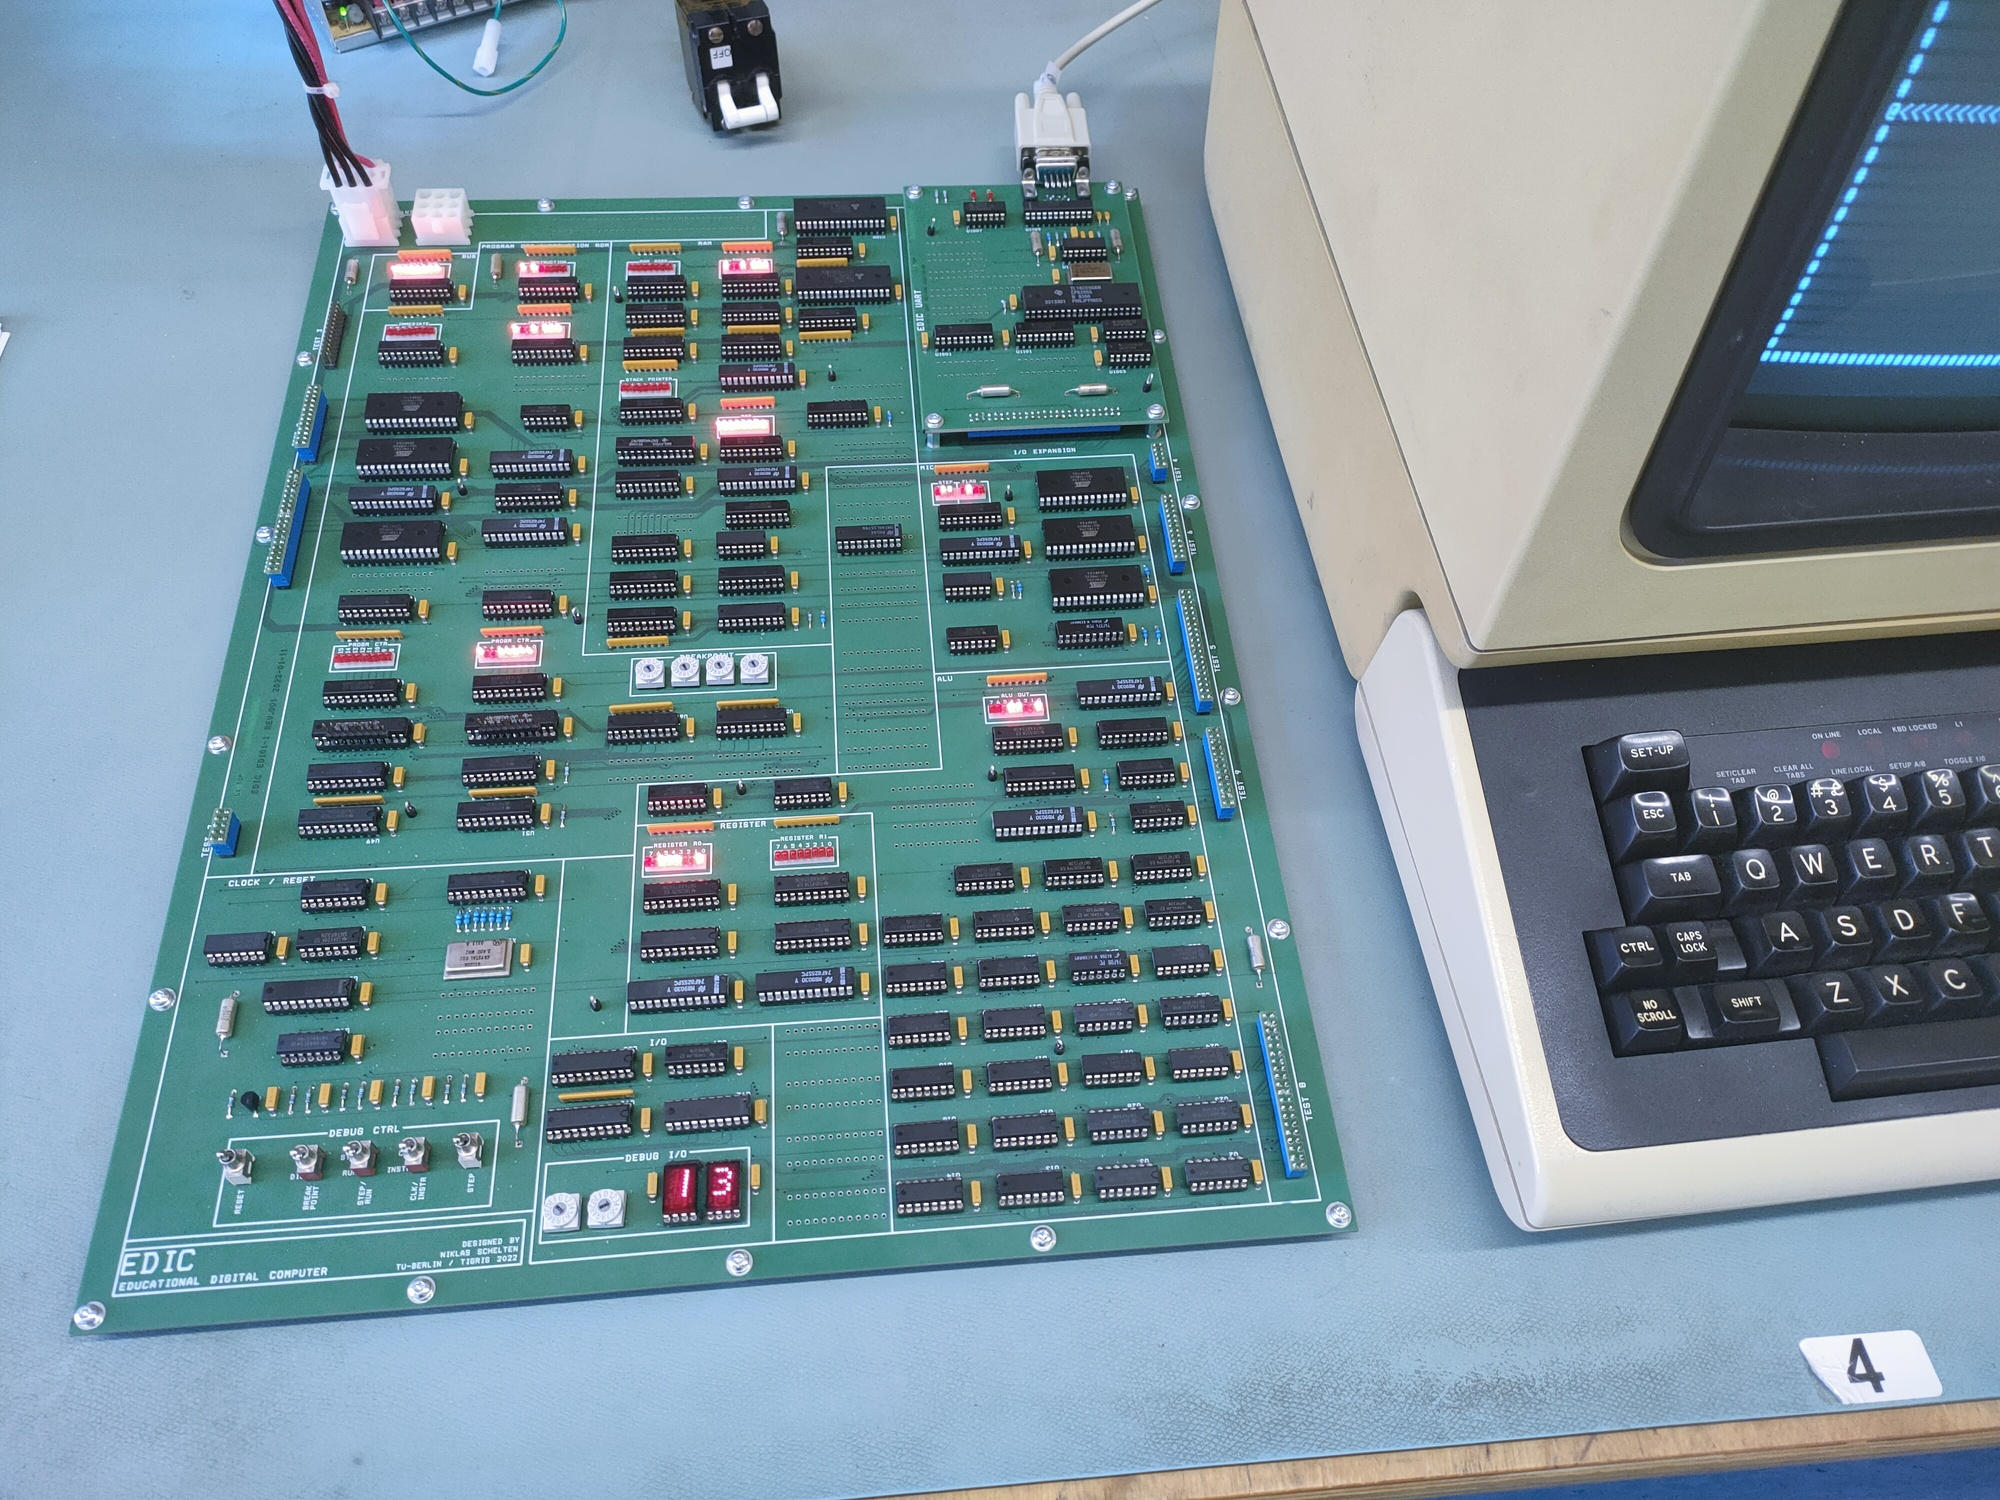
\includegraphics[width=\textwidth]{IMG20220308163628_resize.jpg}
  \caption{The final version of the \gls{EDiC} playing Snake on a VT-100 over an RS-232 I/O card.}
  \label{fig:EDiCSnake}
\end{figure}
\section{Background}
\subsection{Short History on Computing}
The history of computing hardware goes back to ancient times when people used devices like the abacus which simplifies calculations like additions or multiplications.
Starting from the end of the 19th century, analog computers were developed which used continuous physical phenomena to explore complex problems.
One of the first widespread analog computers was created by Sir William Thomson (Lord Kelvin) which predicted tide levels for particular locations by using a set of pulleys and wires. \cite{sep-computing-history}
Even though analog computers could perform very complex operations like solving differential equations \cite{analogDiff} they also had the major drawback that, due to their analog and continues nature, it was not possible to exactly recreate a calculation.

The idea of modern, digital computers was firstly theorized by Alan Turing in his paper \emph{On Computable Numbers} in 1936. \cite{10.1112/plms/s2-42.1.230}
He introduced the notion of a universal (Turing) machine which describes a machine that is provable capable of computing everything that is computable.
All the computers today are as capable as a turing machine which is expressed by calling them \emph{turing complete}.
This is with exception from their finite memory and limited number range.
The first digital computers from the mid 20th century were mechanical or electromechanical machines which combined basic switches like relays and mostly mechanical memory.
As fully electrical computers increased the switching frequencies, a lot of different number formats where emerging:
Opposed to analog computers where one signal, e.g. a voltage, \emph{represents} a value, it now needs to \emph{encode} a value.
In the nowadays common binary system one signal encodes either a 0 or a 1 (for example a low and high voltage) but a lot of different number systems where used like bi-quinary\footnote{Bi-quinary has one quinary signal encoding 0-4 or 5-9 depending on one binary signal encoding a low or high number. This allows two signals to encode a decimal digit similarly to some abacuses.}.

A variety of technologies where developed for fully electric computers like vacuum tubes or transistors.
After using discrete transistors, the advent of \glspl{IC} in the late 50th lead to a rapid acceleration of computer complexity and speed while reducing the power consumption drastically.
The series of \glspl{IC} which is the most relevant to this thesis is the \gls{TTL} 74 series.
It is a successor of one of the first \gls{TTL} \glspl{IC} developed by Texas Instruments in 1964 for military applications: The 5400 series. \cite{ICs}
The 5400 series of \glspl{IC} was specified for a temperature range from \qty{-55}{\celsius} to \qty{+125}{\celsius} and came in a ceramic \gls{SMD} and \gls{DIL} packaging to meet the high requirements of the military and space industries.
Each package included a set of basic logic circuits like 4 2-input NAND gates in the 5400N.
In 1966 the first \glspl{IC} of the 74 series were released which had the same functions but with a reduced temperature rating of \qty{0}{\celsius} to \qty{+70}{\celsius} and often came in plastic packaging for consumer applications.
In contrast to previous \gls{RTL}, these \gls{TTL} \glspl{IC} were capable of higher switching frequencies and lower power consumption due to a second transistor driving the high voltage level.
See \cref{sec:ttl} for a more in depth description of the workings of a \gls{TTL} gate.
As the 74 family of \glspl{IC} became larger with more complex \glspl{IC}, more advanced technologies, such as \gls{CMOS}, were also introduced into the family to further reduce the power consumption or increase the switching speeds.

With further advances in the complexity and integration of computing nodes, the first microprocessors were developed in the 70s with the famous Intel 4004 and 8080 in 1971 and 1974, respectively.
These processors combine all the logic required for a general purpose \gls{CPU} into one \gls{IC} usually exposing interfaces for connecting memories and user \gls{IO} logic.

\subsection{Technology Selection for the \gls{EDiC}}
The design goal for the \gls{EDiC} was to create a \gls{CPU} which aids the teaching of how \glspl{CPU} generally work.
To build a custom \gls{CPU}, many of the above-mentioned technologies were used for computer design, however, not all of them are equally suited for a model \gls{CPU}.
It was decided to use \gls{TTL} \glspl{IC} of the 74 family in the \gls{EDiC} for several reasons:
\begin{itemize}
  \item \emph{Complexity:} The \glspl{IC} of this family are complex enough to make it possible to build complex systems as a general-purpose \gls{CPU} with only about 100 chips.
  On the other hand, each individual \gls{IC} is easy to understand since it is kept quite simple, for example the 7400 has a basic interface of 12 pins for the four 2-input NAND gates plus GND and +5V pins.

  \item \emph{Speed:} In contrast to previous technologies such as electromechanical relays or \gls{RTL}, the 74 series is a lot faster, particularly the 74F subseries which is mainly used in the \gls{EDiC}.
  It is feasible to create complex designs with the 74F series with a clock frequency of several \unit{\mega\hertz}.
  However, at the same time, the clock frequency is not too high, so that special care must be taken when designing the \gls{PCB} which would be the case with higher frequency signals.

  \item \emph{Simplicity:} Working with the \glspl{IC} is fairly easy: No special tools -- except a soldering iron and oscilloscope -- are required to assemble and test the system.
  Especially the usage of sockets for the \glspl{DIP} simplifies the build because no \gls{IC} can overheat while soldering and all the \glspl{IC} can be replaced later on or while testing.
\end{itemize}

In contrast to previous and also later technology, the \gls{TTL} also stands out as the best suited one.
When trying to build a \gls{CPU} out of discrete transistors, not only the logical level needs to be respected but a lot of static and dynamic behavior of the transistors needs to be analyzed.
This complicates the design and prevents students from comprehending the \gls{CPU} on its logical level.
On the other side, more modern technologies became so abstract and complex to use that the comprehension of the internal workings of the \gls{CPU} could also be lost.
For example, when choosing \glspl{FPGA} as the driving technology, the work surrounding the technology quickly becomes more complex than the \gls{CPU} itself.
The \gls{FPGA} \glspl{IC} require special voltage levels and special care with the high frequency clock traces, are hard to solder with small pins, require complex build toolchains, cannot be debugged with an oscilloscope and so on.

Thus, the \gls{TTL} was the ideal technology level for creating a model \gls{CPU} which helps students understanding the workings of \glspl{CPU}.

\subsection{Workings of \gls{TTL}}\label{sec:ttl}
\begin{figure}[t]
  \centering
  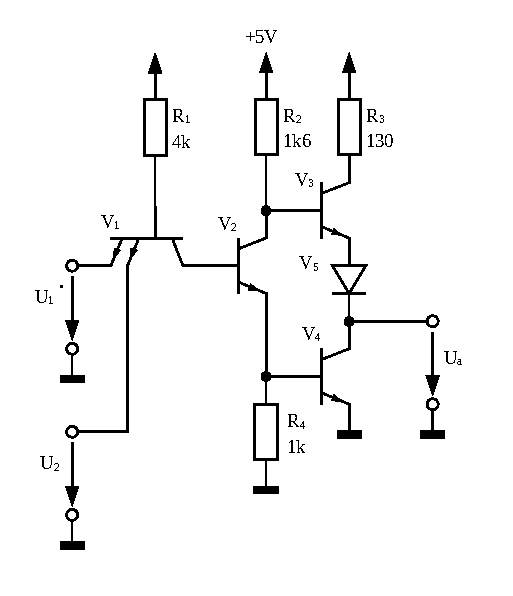
\includegraphics[width=\textwidth]{7400_Circuit.pdf}
  \caption{\gls{TTL} NAND with ``totem-pole'' output stage as in the 7400 \gls{IC}. \cite{7400_Circuit}}
  \label{fig:7400_Circuit}
\end{figure}

\Cref{fig:7400_Circuit} shows the internals of one of the four NAND gates inside the 7400 \gls{IC}.
The multi-emitter transistor $V_1$ functions as the logical NAND gate while the transistors $V_2$, $V_3$ and $V_4$ in combination with the diode $V_5$ form the ``totem-pole'' output stage.
If both inputs are high, a small collector current is drawn by both inputs because $V_1$ is in reverse-active mode.
The current through $R_1$ ``activates'' $V_2$ which in turn ``activates'' $V_4$ due to the current steering effect, where the current flows through the one parallel voltage-stable element with the lowest threshold voltage.
In this case, the current flows through $R_2$, $V_2$ collector-emitter and $V_4$ base-emitter rather than through $V_3$ collector-emitter, $V_5$ and $V_4$ collector-emitter.
Therefore, $V_4$ drives the output with a low voltage.

If one of the inputs is low, on the other hand, the current steering effect turns off $V_2$ since the current flows through $R_1$ and $V_1$ base-emitter rather than $R_1$, $V_1$ base-collector $V_2$ base-emitter and $R_4$.
Hence, the above-mentioned current steering effect on the output stage no longer takes effect and $V_3$ drives the output high through the diode $V_5$.

The advantage of this ``totem-pole'' output stage in comparison to a more simple output stage with the collector of $V_2$ effectively being the output is, that a very low output resistance can be achieved (only the small $R_3$) which allows the output to drive more inputs of other logic gates.
Additionally, the speed is drastically increased because the high output is actively driven instead of pulled up via a resistor as in \gls{RTL}.
However, the voltage drop over $V_3$ and $V_5$ also have the effect that the high output voltage is only about \qty{3.5}{\volt} in contrast to the simpler approach where almost \qty{5}{\volt} can be achieved.


\section{Thesis Structure}
Firstly, the following \cref{cha:architecture} will give an in-depth explanation of the \gls{CPU} architecture.
It includes an analysis of the design goals and explanations of how they can be achieved.
The individual modules are described as well as how they work together to execute any instruction.

Foccusing on usability, the \cref{cha:software} gives an overview of the software environment which eases the development of programs for the \gls{EDiC}.
Furthermore, it also features a tool with which the microcode for instructions can be changed, or new instructions can be added which is especially important looking at the educational purpose of the model \gls{CPU}.

Subsequently, \cref{cha:fpga} gives a short background to \glspl{FPGA} and then covers all the important aspects of the \gls{FPGA} model which was created to verify the architecture.
With a chip-level \gls{FPGA} implementation it was possible to not only verify the architecture but also the schematic of the \gls{EDiC} on the logical level.

In \cref{cha:hardware} the hardware design is finally detailed.
Besides an explanation of the schematics (attached in \cref{cha:schem}), the chapter also contains  information on the development process of the \gls{PCB} design.

After the \gls{PCB} was designed and produced, the process of testing the components and verifying all instructions is shown in \cref{cha:eval}.

A final conclusion and possibilities for further work are then given in \cref{cha:conclusion}.

% !TEX root = ../thesis.tex

\chapter{Previous Work}\label{cha:prev}
This chapter provides an overview of what my workings on the initial \gls{CPU} included.

\section{Design Goal}
My initial goal was to design a \gls{CPU} from scratch without explicitly looking at how other architectures had solved occurring problems.
This meant I was to rely on the knowledge I had achieved until then and came up with the following specifications I wanted my \gls{CPU} to fulfill:
\paragraph{8 bit bus width}
Most current era \glspl{CPU} employ a 32 bit or 64 bit bus to handle large numbers and large amounts of data.
It was clear to me that I needed to settle for a smaller bus when building a \gls{CPU} by hand.
Some early \glspl{CPU} worked with only 4 bits but to not be as limited I finally chose to use an 8 bit bus.
\paragraph{Datapath Architecture - Multicycle CISC}
In most \glspl{CPU} an instruction is not done in one clock cycle but it is divided into several steps that are done in sequence.
There are two general approaches that are called \emph{Multicycle} and \emph{Pipelining} \cite{PattersonDavid2016RuRD}.
Multicycle means that all the steps of one instruction are performed sequentially and a new instruction is only dispatched after the previous instruction is finished.
This is usually used when implementing \glspl{CISC}, where one instruction can be very capable \cite{chen_novick_shimano_2000}.
For example a add instruction in \gls{CISC} could fetch operands from memory, execute the add and write the result back to memory.
\glspl{RISC} on the other hand would need independent instruction to load operands from memory into registers, do the addition and write the result back to memory.

In Pipelining there a fixed steps each instruction goes through in a defined order and the intermediate results are stored in so called pipeline registers.
Each pipeline step is constructed in such a way that it does not intervene with the others.
Therefore, it is possible to dispatch a new instruction each cycle even though the previous instruction is not yet finished.
A typically 5-step pipeline would consist of the following steps \cite{PattersonDavid2016RuRD}:
\begin{enumerate}
  \item \textbf{Instruction Fetch}: The instruction is retrieved from memory and stored in a register.
  \item \textbf{Instruction Decode}: The fetched instruction is decoded into control signals (and instruction specific data) for all the components of the \gls{CPU}.
  \item \textbf{Execute}: If arithmetic or logical operations are part of the instruction, they are performed.
  \item \textbf{Memory Access}: Results are written to the memory and/or data is read from memory.
  \item \textbf{Writeback}: The results are written back to the registers.
\end{enumerate}
However good the performance of a pipelined \gls{CPU} is, it also comes with challenges.
Those include a greater resource usage because all intermediate results need to be stored in pipeline registers.
Additionally, branch instructions\footnote{Branch Instructions change the program counter and with that the location from which the next instruction is to be fetched. This is required for conditional and looped execution.} pose a great challenge because at the moment, the \gls{CPU} execute the branch the next instructions have already been dispatched.
This means that the pipeline needs to be flushed (i.e. cleared), performance is lost and more logic is required.
It also noteworthy that branch prediction and pipeline flushes can be quite vulnerable as recently shown in CVE-2017-5753 with the Spectre bug \cite{CVE-2017-5753}.

Therefore, I decided to build my \gls{CPU} as a Multicycle \gls{CISC}.

\paragraph{Single-Bus Oriented}
The decision for a Multicycle \gls{CPU} also enabled the architecture to be single-bus oriented.
This means that all modules (e.g. the \gls{ALU} and the memory) are connected to a central bus for data transfer.
The central bus is then used as a multi-directional data communication.
To allow this in hardware, all components that drive the bus (i.e. ``send'' data) need to have a tri-state driver.
A tri-state driver can either drive the bus with a defined `0' or `1' or high impedance which allows other tri-state drivers on the same bus to drive it.
That way an instruction which fetches a word from the memory from an address stored in a register and stores it in a register could consist of the following steps:
\begin{enumerate}
  \item Instruction Fetch
  \item Instruction Decode
  \item Memory Address from register over \emph{bus} to memory module
  \item Memory Access
  \item Data from memory module over \emph{bus} to register
\end{enumerate}
With such an architecture it is possible to avoid large multiplexers and keep the overall architecture simple.

\section{Implementation}
As mentioned above, the \gls{CPU} is divided into multiple modules which are only connected over the bus apart from control signals and one other exception.
\subsection{Modules}
The original design was split into 7 independent modules of varying complexity.
\subsubsection{\glsxtrfull{ALU}}
\begin{table}
  \centering
  \renewcommand{\arraystretch}{1.25}
  \caption{Summary of the available alu operations.}
  \label{tab:aluOp}
  \begin{tabularx}{.8\textwidth}{ |c|c|c||X| }
    \hline
    aluOp[1] & aluOp[0] & aluSub & Resulting Operation\\\hline\hline
    0 & 0 & 0 & ($A + B$) Addition \\\hline
    0 & 0 & 1 & ($A - B$) Subtraction \\\hline
    0 & 1 & 0 & ($A \land B$) AND \\\hline
    0 & 1 & 1 & ($A \land \overline{B}$) \\\hline
    1 & 0 & 0 & ($A \veebar B$) XOR \\\hline
    1 & 0 & 1 & ($\overline{A \veebar B}$) XNOR \\\hline
    1 & 1 & 0 & ($A \gg B$) logical shift right \\\hline
    1 & 1 & 1 & ($A \ll B$) logical shift left \\\hline
  \end{tabularx}
\end{table}
The \gls{ALU} is capable of 4 different operations plus inverting the $B$ input for two's complement subtraction.
Therefore, there are three control signals which control the operation: two alu-operation bits plus one subtract bit.
The $B$ input is XORed with the aluSub bit which results in the $B$ input being inverted when aluSub is `1' and otherwise $B$ remains the same.
The aluSub bit is also connected to the carry input of the adder and with that, results in a two's complement subtraction.
All possible operations are shown in \cref{tab:aluOp}.
\begin{figure}[t]
  \centering
  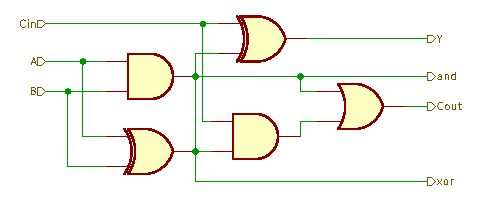
\includegraphics[width=\textwidth]{full_adder.pdf}
  \caption{1 bit full adder with the usual A, B and Carry inputs and Y and Carry outputs as well as the XOR and AND outputs.}
  \label{fig:full_adder}
\end{figure}
The adder is a simple ripple carry adder for its simplicity and the XOR and AND operation from the half-adders are also used as the logic operations.
A complete 1 bit full-adder is shown in \cref{fig:full_adder}.

\begin{figure}[p]
  \centering
  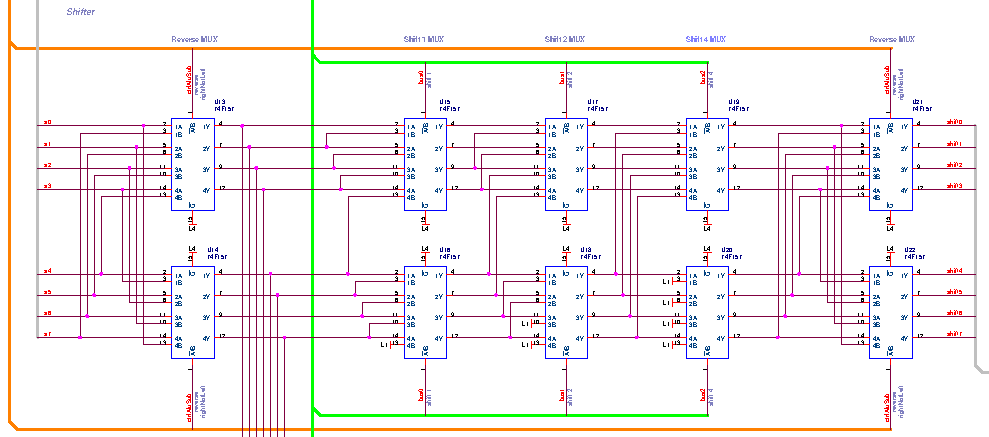
\includegraphics[width=\textheight, angle=90]{barrel_shifter.pdf}
  \caption{8 bit bidirectional barrel shifter.}
  \label{fig:barrel_shifter}
\end{figure}
It was desirable to include a barrel shifter to have the possibility to improve multiply operation with a shift and add approach instead of repeated addition.
The barrel shifter works by 3 consecutive multiplexers to shift by 1, 2 or 4 bit to the right that are controlled by the first 3 bit of the (not inverted) $B$ input.
To also allow shifting to the left there is one multiplexer before the three shift multiplexers to invert the order of bits and another one after the shifting to reorder the bits.
In \cref{fig:barrel_shifter} a bidirectional barrel shifter implemented with the \texttt{74F157} is visualized. The \texttt{74F157} implements four 2 to 1 multiplexer and, therefore, 2 chips are needed for a full 8 bit 2 to 1 multiplexer.

The multiplexed result is stored in an 8 bit \gls{ALU} result register.
For conditional execution the \gls{ALU} includes two flags: Not Zero (at least one bit is one) and negative (the \gls{MSB}).

\subsubsection{Register File}
As is typical with \glspl{CISC} the \gls{CPU} does not need many general purpose registers and the register file can be kept simple with only two registers.
The register file has one write port (from the bus) and two read ports of which one reads to the bus and the other is directly connected to the $A$ input of the \gls{ALU}.
\subsubsection{Control Logic}\label{ssec:cl}
The control logic's job is to decode the current instruction and provide all the control signals for each cycle for any instruction.
For keeping track which cycle of each instruction is currently executing a 3 bit synchronous counter is needed.
Each control signal could be derived by a logical circuitry with 13 inputs: 8 bits instruction, 2 bits \gls{ALU} flags and 3 bits cycle counter.
However, designing these logic circuits is a lot of work, takes up a lot of space and cannot be changed easily later on. (For example when finding a bug in one instruction)
Therefore, an \gls{EEPROM} is used where the 13 bits that define one cycle of one specific instruction are used as addresses.
The control signals then are the data bits of the word that is stored at the specific address in the \gls{EEPROM}.

The first two cycles of each instruction need to be taken in special consideration because the instruction register is not yet loaded with the next instruction, because it is still being fetched and decoded.
However, the instruction fetch and decode are always the same for each instruction, which means that all memory locations where the cycle counter is equal to 0 or 1 (the first two instructions) are filled with the control signals for an instruction fetch and decode.
\subsubsection{Memory}
The memory module contains the main memory of the \gls{CPU} in form of an asynchronous \gls{SRAM} and the instruction memory as an \gls{EEPROM}.
This way a new program can be loaded into the \gls{CPU} by reprogramming the \gls{EEPROM}.
Both the \gls{SRAM} and the \gls{EEPROM} have their data lanes connected to the bus for reading from and writing to the memory.
The address is controlled via an \gls{MAR} from the bus.
\subsubsection{Program Counter}
The program counter is a special register with two main functionalities:\\
Usually it increments by one after each instruction.
However, when a branch is executed it needs to load the branch address from the bus.
For this an 8 bit increment similar to the cycle counter from the Control Logic \cref{ssec:cl} is multiplexed with the bus and used as the input data for the register.
\subsubsection{Input \& Output}
This first version of the \gls{CPU} included very rudimentary I/O logic.
For input it provides an 8 bit DIP-Switch connected to the bus and for output there is a register with a 2 digit 7-segment display.
\subsubsection{Clock \& Reset}
The function of the clock module is threefold:\\
It provides a clock for the whole \gls{CPU} while also providing an active-low reset for some of the registers to provide a defined starting condition.
The clock has two modes. One to run continuously and another where the clock can be manually advanced.
Additionally, there is a halt instruction which stops the \gls{CPU} clock until a button is pressed.
\subsection{FPGA Simulation}
The goal of the \gls{FPGA} simulation is to proof the general workings of the \gls{CPU} architecture.
There was no attempt made to provide a chip-level simulation of the hardware build but rather to provide a top-level behavioral model.
The chosen development environment is the AMD - Xilinx Vivado \cite{vivado} as it is freely available and provides an advanced simulation environment while providing the possibility to synthesize for relatively cheap \glspl{FPGA}.

\subsection{Hardware Build}

The clock circuit is heavily inspired by the clock module of the above mentioned YouTube series by Ben Eater \cite{eater_clock}.
% !TEX root = ../thesis.tex
\chapter{Design Adaptations}\label{cha:designChanges}
For building the \gls{EDiC} the goal was to keep to the same basic infrastructure of the first version \gls{CPU}.
However, many bugs and problems that occurred in the building of it should be addressed and avoided.
Furthermore, the \gls{CPU} should be extended with some important features that were not implemented in the first version.
\section{General Improvements}\label{sec:improvements}
There are several design decisions, especially in the hardware built, which caused problems or could have caused problems in certain circumstances.
\paragraph{LED Driver}
First of all, all \glspl{LED} were directly connected to the logic wires.
This does work but the outputs of all logic \glspl{IC} have a limited current they can provide.
For example, the \emph{74LS245} is rated for maximum \qty{20}{\uA} for high-level output and \qty{-200}{\micro\ampere} for an low-level output \cite{74ls245}.
The way the \glspl{LED} were connected in the first \gls{CPU} they use only current when the logic \gls{IC} outputs a high-level voltage which is rated for \nicefrac{1}{10} the output current.
When connecting more \glspl{IC} and one \gls{LED} the maximum current can easily be exceeded.
Therefore, all \glspl{LED} of the \gls{EDiC} are powered with an additional inverting driver, the \emph{74ABT540} which is rated for \qty{50}{\uA} in both directions \cite{74abt540}.
\paragraph{Register \gls{IC}}
\begin{figure}[t]
  \centering
  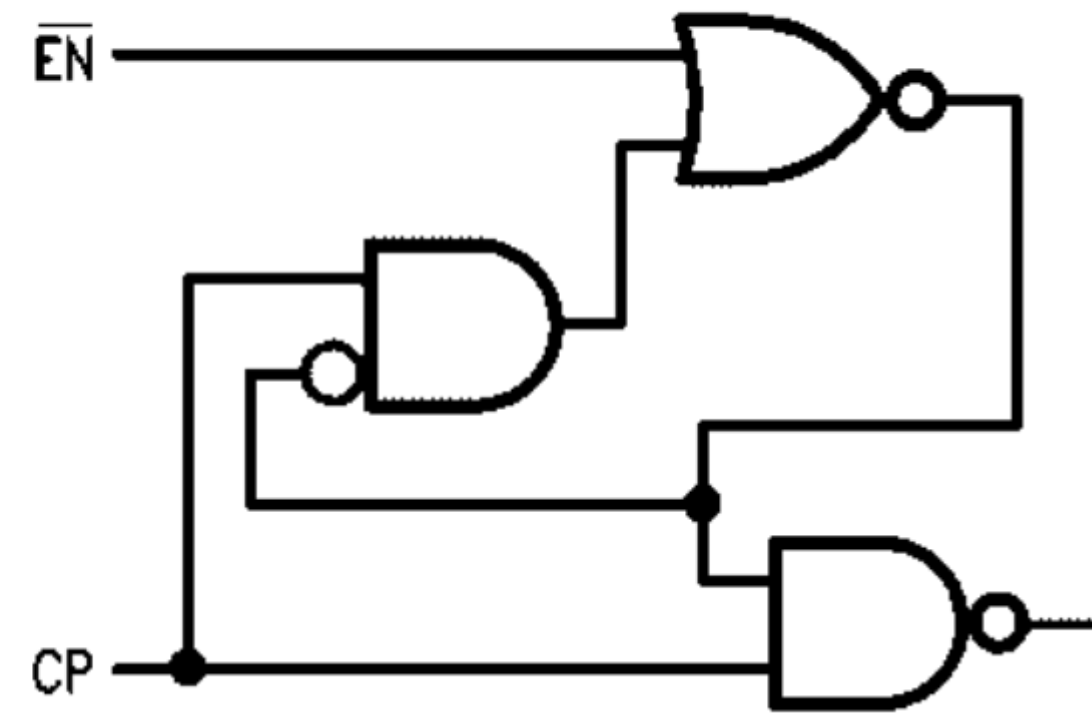
\includegraphics[width=.6\textwidth]{ce.png}
  \caption{Clock Enable circuit of the \emph{74F825} \gls{IC} \cite{74f825}.}
  \label{fig:clockEnable}
\end{figure}
% A basic 1 bit register
The 74 series of logic \glspl{IC} feature many different registers.
The most basic register \gls{IC} has $n$ D-type flip-flops with respective data inputs and outputs plus one common clock input.
On each rising edge of the clock the flip-flops capture the input values and hold them until the next rising edge of the clock.
However, often it is required that a register does not capture on every rising edge of the clock.
This is done with an additional input, called clock enable.
In the first version of the \gls{CPU} the clock inputs of the registers that needed clock enable were connected to the output of an AND gate of the clock and a control bit.
This has the major drawback that glitches of the enable control signal can propagate to the clock input of the register when the clock is currently high.
There are two widely used alternatives to the simple AND gate:
The enable input can be used as the select input for an multiplexer to the data input of the flip flop, where it multiplexes between the actual input and the current output.
This allows the flip-flop to always capture data but when the enable input is inactive, it recaptures the current output.
The drawbacks are that each bit of the register needs a multiplexer at the input and secondly that the flip-flops draw power on every clock pulse, even though no data is captured.
The \emph{74F825} logic \gls{IC} solves this with the circuit shown in \cref{fig:clockEnable}.
When the $\overline{\text{EN}}$ input is low, the CP input is NAND gate on the right passed the negated CP through\footnote{The internal flip-flops of the \emph{74F825} are negative edge triggered}.
When the $\overline{\text{EN}}$ input is high, on the other hand, the output does not change.
This circuit prevents the $\overline{\text{EN}}$ to trigger a falling edge (which would trigger the flip-flops) on the CP output.
However, when the $\overline{\text{EN}}$ goes high while the CP input is high, then the output also goes high.
This is not directly a problem because the flip-flops only trigger on falling edges but is the reason for timing requirements on the $\overline{\text{EN}}$ input which are discussed in more detail in \cref{sec:timing}.
\begin{figure}[t]
  \centering
  \begin{subfigure}[b]{.45\textwidth}
    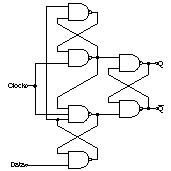
\includegraphics[height=7.5cm]{DFlipFlop.pdf}
    \subcaption{Classical D-type flip-flop built out of three $\overline{\text{SR}}$ NAND latches \cite{DFlipFlop}.}
  \end{subfigure}%
  \hspace{.05\textwidth}
  \begin{subfigure}[b]{.45\textwidth}
    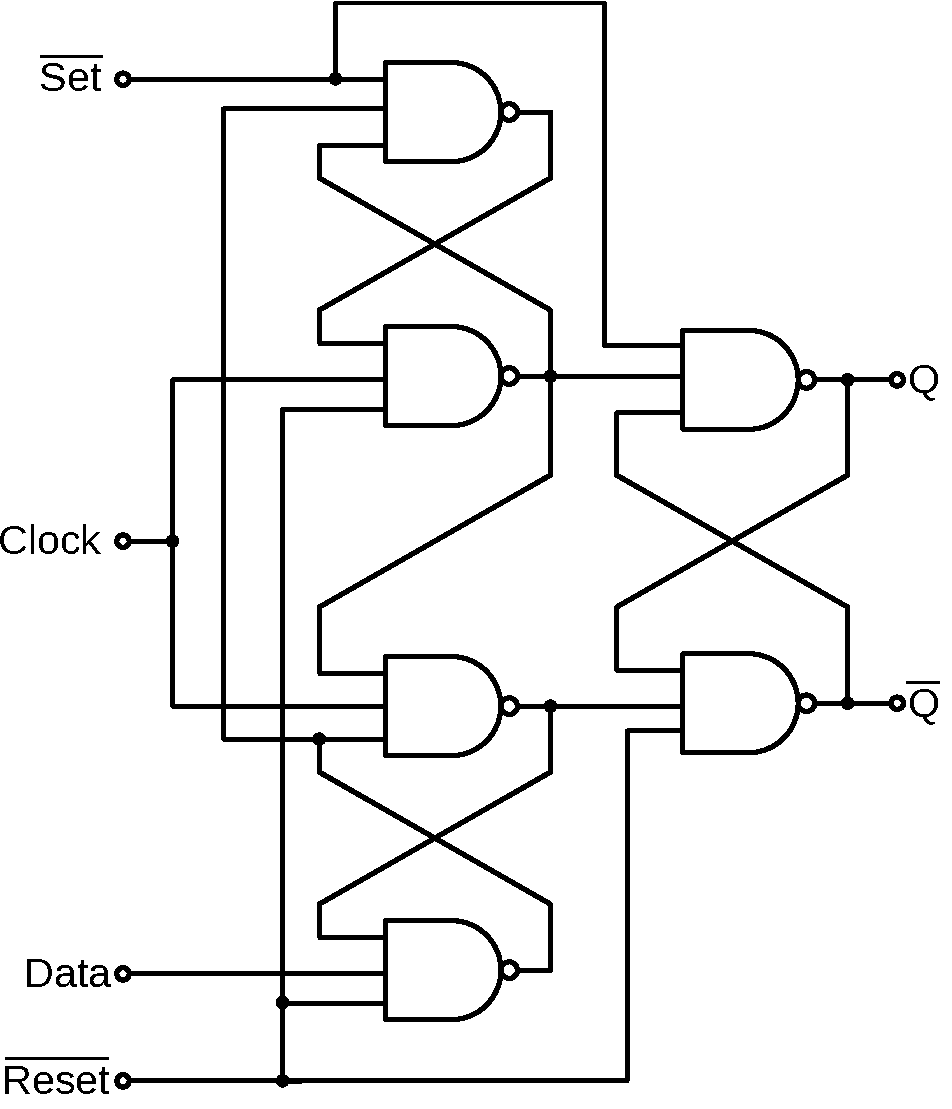
\includegraphics[height=7.5cm]{DFlipFlopClearSet.pdf}
    \subcaption{D-type flip-flop modified to support $\overline{\text{Clear}}$ and $\overline{\text{Set}}$ \cite{DFlipFlopClearSet}.}
  \end{subfigure}
  \caption{Comparison of D-type flip-flops with and without $\overline{\text{Clear}}$ and $\overline{\text{Set}}$.}
  \label{fig:clearSet}
\end{figure}
As the registers store the current state of execution, it is required that the registers start up to a known state.
Therefore, some registers feature a clear input (or set input) which forces all flip-flops to 0 (or 1).
This is usually accomplished by modifying the classical D-type flip-flop to allow for setting and resetting the internal $\overline{\text{SR}}$ NAND latches as shown in \cref{fig:clearSet}.

The third feature that may be important is a three-state output which allows the register to be directly connected to a bus.
It is accomplished by adding a tri-state output driver to the outputs of the flip-flops.

The logic \gls{IC} that was chosen for the \gls{EDiC} because it has all three features and is 8 bits wide is the \emph{74F825}.
\section{16bit Addresses}
\section{Memory Mapped IO}
\section{Stack Implementation}
\section{Debugging and Breakpoint}
% !TEX root = ../thesis.tex
\chapter{Software Development Environment}\label{cha:software}
When just providing the hardware, the \gls{CPU} can hardly be used.
It is possible to write programs by hand by writing single bytes to the \glspl{EEPROM} that hold the program.
However, it is quite infeasible to write complex programs this way.
Even more extreme is content of the \glspl{EEPROM} holding the micro code, i.e. that decode the instruction depending on the instruction cycle and \gls{ALU} flags.

Therefore, the \gls{EDiC} comes with two main software utilities that form the Software Development Environment.

\section{Microcode Generation}
\begin{listing}[t]
  \inputminted[linenos,
    breaklines,
    frame=leftline,
    xleftmargin=20pt,
  ]{TypeScript}{src/microcode.ts}
  \caption{Schema of the Microcode Definition CSON-File \cite{CSON} as a TypeScript \cite{TS} Type definition.}
  \label{lst:micrcode_schema}
\end{listing}
The goal is to define all the available instructions and what they perform in which instruction step and then have a program automatically generate the bit-files for the \gls{EEPROM}.
This approach allows to easily make changes to the existing microcode if a bug was found or a new instruction should be added.
The file format which defines the microcode has to be human and machine readable as it should be easily edited by hand and also be read by the tool that generates the bit-files.
A very common file format for tasks like this is \gls{JSON} \cite{JSON} which is widely used in the computer industry.
Besides basic types as strings and numbers, it allows basic arrays with square brackets (\texttt{[]}) and objects with curly braces (\texttt{\{\}}).
Each object contains key value pairs and everything can be nested as desired.
For the \gls{EDiC} microcode generation \gls{CSON} was used which is very similar to \gls{JSON} but is slightly easier to write by hand because its syntax is changed a bit:
\begin{itemize}
  \item It allows comments which is extensively used to ease the understanding of individual instruction steps
  \item Braces and commas are not required
  \item Keys do not require string quotation marks
\end{itemize}
The schema for the file describing the microcode is shown in \cref{lst:micrcode_schema}.
The file is an object with three key, value pairs:
\paragraph{Signals}
\begin{listing}[h!]
  \begin{minted}[linenos,
    breaklines,
    frame=leftline,
    xleftmargin=20pt,
  ]{CoffeeScript}
  {
    name: 'reg0NWE'
    noOp: 1
  }
  \end{minted}
  \caption{Example of a control signal definition for the microcode generation.}
  \label{lst:mc_signals}
\end{listing}
The signals array consists of Objects that define the available control signals and the default value of the control signal.
\Cref{lst:mc_signals}
defines the \emph{not write enable signal for register 0} control signal and defines the default state as high.
This means, when this control signal is not specified it will stay high and, therefore, register 0 will not be written.

\paragraph{InstructionFetch} This array defines the steps that are performed at the beginning of each instruction to fetch the new instruction and decode it.
Each object represents one step and consists of key value pairs that define one control signal.
\begin{listing}[h!]
  \begin{minted}[linenos,
    breaklines,
    frame=leftline,
    xleftmargin=20pt,
  ]{CoffeeScript}
    instructionFetch: [
      { # write instruction
        memInstrNWE: 0
      }
      { # increment PC
        memPCNEn: 0
        memPCLoadN: 1
      }
    ]
  \end{minted}
  \caption{Definition of the instruction fetch and decode steps for the microcode generation.}
  \label{lst:mc_instrFetch}
\end{listing}

For example \cref{lst:mc_instrFetch} he first step specifies only the \emph{instruction not write enable} to be low and with this write the instruction into the instruction register.
Secondly, the \gls{PC} is incremented by setting \emph{PC not enable} to low and \emph{PC not load} to high.
\paragraph{Instructions} The instructions are an array of all available instructions.
Each instruction is defined as an \texttt{op} code, which is the 8 bit instruction in binary format.
However, if it was only possible to define the 8 bit as 0s and 1s instructions which only differ in the register used would need to be specified separately which is very error prone.
Therefore, it is allowed to specify the bit that specifies if register 0 or 1 is used to be set to \texttt{'r'} or \texttt{'s'} and then multiple instructions are generated.
Each instruction then The \texttt{cycles} array define the steps each instruction does in the same way as the \texttt{instructionFetch} array does.
However, as the value of individual control signals may depend up on which register is specified in the op code, it is also possible to specify \texttt{'r'}, \texttt{'!r'}, \texttt{'s'} or \texttt{'!s'}.

\begin{listing}[h!]
  \begin{minted}[linenos,
    breaklines,
    frame=leftline,
    xleftmargin=20pt,
  ]{CoffeeScript}
  {
    op: '1111100r' # r = imm
    cycles: [
      { # imm to bus to r
        reg0NWE: 'r'
        reg1NWE: '!r'
        memInstrNOE: 0
      }
    ]
  }
  \end{minted}
  \caption{Definition of the move immediate to register instruction for the microcode generation.}
  \label{lst:mc_movImm}
\end{listing}
\Cref{lst:mc_movImm} defines the move immediate to register instruction for both register at the same time.
The \emph{instruction immediate not output enable} is low and either register 0 or register 1 is written to.
This definition would be equal to \cref{lst:mc_movImmDuplicate}.
\begin{listing}[h!]
  \begin{minted}[linenos,
    breaklines,
    frame=leftline,
    xleftmargin=20pt,
  ]{CoffeeScript}
  [
    {
      op: '11111000' # r0 = imm
      cycles: [
        { # imm to bus to r0
          reg0NWE: 0
          reg1NWE: 1
          memInstrNOE: 0
        }
      ]
    }
    {
      op: '11111001' # r1 = imm
      cycles: [
        { # imm to bus to r1
          reg0NWE: 1
          reg1NWE: 0
          memInstrNOE: 0
        }
      ]
    }
  ]
  \end{minted}
  \caption{Definitions of the move immediate to register instruction for each register separately for the microcode generation.}
  \label{lst:mc_movImmDuplicate}
\end{listing}

This example is quite simple, however, instructions with two registers as arguments would result in four times the same definition and duplication can always result in inconsistencies.
The same idea is also used for the \gls{ALU} operations.
The \gls{ALU} operations are not generated by the microcode but are rather the three least significant bits of the instruction.
Therefore, all instructions using the \gls{ALU} can have the exact same control signals stored in the microcode \gls{EEPROM}.
To avoid 8 definitions of the same instructions, the op code can contain \texttt{'alu'} and all 8 instructions are generated.
\begin{listing}[h!]
  \begin{minted}[linenos,
    breaklines,
    frame=leftline,
    xleftmargin=20pt,
  ]{CoffeeScript}
  {
    op: '000rsalu' # r = r x s (alu)
    cycles: [
      { # r x s into alu
        aluYNWE: 0
        reg0BusNOE: 's'
        reg1BusNOE: '!s'
        regAluSel: 'r'
      }
      { # alu into r
        aluNOE: 0
        reg0NWE: 'r'
        reg1NWE: '!r'
      }
    ]
  }
  \end{minted}
  \caption{Definition of the alu operation with two register arguments for the microcode generation.}
  \label{lst:mc_aluRS}
\end{listing}
\Cref{lst:mc_aluRS} for example defines the alu operation with two registers and defines all 32 instructions with the op codes \texttt{'00000000'} to \texttt{'00011111'}.

\begin{listing}[h!]
  \begin{minted}[linenos,
    breaklines,
    frame=leftline,
    xleftmargin=20pt,
  ]{CoffeeScript}
  {
    op: '1010flag' # pc := imm
    cycles: [
      { # imm to pc
        memPCNEn: 0
        memPCLoadN: 0
        memPCFromImm: 1
      }
    ]
  }
  \end{minted}
  \caption{Definition of the branch instructions.}
  \label{lst:mc_branch}
\end{listing}
There is one final specialty built into the Microcode Generator:
The \gls{EDiC} has a branch instruction which is either executed or treated as a no-operation depending on the current state of the \gls{ALU} flags.
For all other instructions, the flags are ignored and always executed\footnote{Meaning that all memory locations for the instruction and step counter, no matter the \gls{ALU} flags, store the operation.}.
For this special instruction, the last for bits replaced with \texttt{flag} define at which state of the \gls{ALU} flags, the branch should be executed.
The possible conditions are heavily inspired by the conditional execution of ARM \glspl{CPU}\cite{armCond} as the \gls{ALU} flag architecture is very similar.
The possible values for the \texttt{flag} field and their meanings are listed in \cref{tab:mc_flagMeanings}.
Especially for a \gls{CPU} with only 8 bits it is important to support unsigned and signed operations and with a complex microcode it is no problem to support all the different branch instructions and with it facilitate the application design.
\begin{table}
  \centering
  \renewcommand{\arraystretch}{1.25}
  \caption{All available branch instructions with their op-code and microcode translation based on the \gls{ALU} flags explained in \cref{sec:aluFlags}.}
  \label{tab:mc_flagMeanings}
  \begin{tabularx}{\textwidth}{ |c|l|l|X| }
    \hline
    \texttt{flag} (OP-Code) & Assembler Instruction                & \gls{ALU} flags                 & Interpretation   \\\hline\hline
    \texttt{0000}           & \texttt{jmp}/\texttt{bal}/\texttt{b} & Any                             & Always           \\\hline
    \texttt{0001}           & \texttt{beq}                         & \texttt{Z==1}                   & Equal            \\\hline
    \texttt{0010}           & \texttt{bne}                         & \texttt{Z==0}                   & Not Equal        \\\hline
    \texttt{0011}           & \texttt{bcs}/\texttt{bhs}            & \texttt{C==1}                   & Unsigned $\geq$  \\\hline
    \texttt{0100}           & \texttt{bcc}/\texttt{blo}            & \texttt{C==0}                   & Unsigned $<$     \\\hline
    \texttt{0101}           & \texttt{bmi}                         & \texttt{N==1}                   & Negative         \\\hline
    \texttt{0110}           & \texttt{bpl}                         & \texttt{N==0}                   & Positive or Zero \\\hline
    \texttt{0111}           & \texttt{bvs}                         & \texttt{V==1}                   & Overflow         \\\hline
    \texttt{1000}           & \texttt{bvc}                         & \texttt{V==0}                   & No overflow      \\\hline
    \texttt{1001}           & \texttt{bhi}                         & \texttt{C==1} and \texttt{Z==0} & Unsigned $>$     \\\hline
    \texttt{1010}           & \texttt{bls}                         & \texttt{C==0} or \texttt{Z==1}  & Unsigned $\leq$  \\\hline
    \texttt{1011}           & \texttt{bge}                         & \texttt{N==V}                   & Signed $\geq$    \\\hline
    \texttt{1100}           & \texttt{blt}                         & \texttt{N!=V}                   & Signed $<$       \\\hline
    \texttt{1101}           & \texttt{bgt}                         & \texttt{Z==0} and \texttt{N==V} & Signed $>$       \\\hline
    \texttt{1110}           & \texttt{ble}                         & \texttt{Z==0} or \texttt{N!=V}  & Signed $\leq$    \\\hline
    \texttt{1111}           & -                                    & Any                             & Never (Not used) \\\hline
  \end{tabularx}
\end{table}

\section{Assembler}
The second software that is probably even more important is the assembler.
An assembler translates human readable instructions into the machine code, i.e. the bits that are stored in the instruction \glspl{EEPROM}.
For the \gls{EDiC} each instruction is 24 bits wide, with 8 bits instruction op code and 8 or 16 bits immediate value.
Even though assemblers usually only translate instructions one for one, they can have quite advanced features.
With an assembler, the programmer is no longer required to know the specific op codes for all instructions and set individual bits of the instructions which is very error prone.
The assembler for the \gls{EDiC}, therefore, allows easier programming with a simple text-based assembly syntax similar to the well-known ARM syntax.
\begin{listing}
  \inputminted[linenos,
    breaklines,
    frame=leftline,
    xleftmargin=20pt,
  ]{ARM}{src/prng.s}
  \caption{\gls{PRNG} written in the \gls{EDiC} Assembler.}
  \label{lst:asm_prng}
\end{listing}

\begin{listing}
  \inputminted[linenos,
    breaklines,
    frame=leftline,
    xleftmargin=20pt,
  ]{ARM}{src/prng_out.s}
  \caption{The output of the \gls{PRNG} of \cref{lst:asm_prng}. The first 16 bits are the memory address, then 8 bits for the instruction op-code and 16 bits for the instruction immediate and for reference the original instruction with variables replaced.}
  \label{lst:asm_prng_out}
\end{listing}

\Cref{lst:asm_prng,lst:asm_prng_out} show the translation that the assembler does where \cref{lst:asm_prng} shows the assembler program that is written by any programmer and \cref{lst:asm_prng_out} summarizes what values are stored in the program \gls{EEPROM}.

\subsection{Available Instructions}
First of all, this section summarizes all available instructions and which parameters they take.
All instructions start with the operation and then up two parameters separated by a comma.

There are four different parameter types.
It can either be a register specified as \texttt{r0} or \texttt{r1}.
The register value can also be passed as the address to a memory operation with \texttt{[r0]}.

Immediate values can also be specified as value or as address with brackets around the immediate value.
However, the syntax for immediate values is more complex, as the assembler can parse decimal (positive and negative) as well as hexadecimal numbers.
Additionally, variables can be used which are further explained in \cref{sec:variables}.
When specifying a value, the immediate can range between -127 and 255 (two's complement and unsigned) and when used as an address it can range between 0 and 0xfffe (65534). The upper limit is not 0xffff because that address is reserved for the return address and should not be overwritten.
\paragraph{\gls{ALU} Instructions} The following \gls{ALU} instructions are available:
\begin{multicols}{4}
  \begin{itemize}
    \item add
    \item sub
    \item and
    \item eor
    \item xor
    \item xnor
    \item lsr
    \item lsl
  \end{itemize}
\end{multicols}
\gls{ALU} instructions always take two parameters. The first parameter is the left hand side operand and the register where the result is stored in and the second parameter is the right hand side operand.
\begin{itemize}
  \item Two registers

  \qquad\texttt{sub r0, r1} does: $r_0:=r_0-r_1$
  \item One register and one register as memory address

  \qquad\texttt{lsr r1, [r0]} does: $r_1:=r_1\gg\text{mem}[r_0]$
  \item One register and an immediate value

  \qquad\texttt{and r0, 0x0f} does: $r_0:=r_0\xor 15$
  \item One register and an immediate value as memory address

  \qquad\texttt{add r1, [0x0542]} does: $r_1:=r_1+\text{mem}[1346]$
\end{itemize}
All of the \gls{ALU} instructions can have an `s' as suffix which has the effect that the result of the operation is not written to the first operand.
This is useful when a calculation is only performed to update the \gls{ALU} flags but the register value is used later on.
This results in a special \gls{ALU} instruction: \texttt{cmp} which is an alias to \texttt{subs} which is typically used to compare to values and perform a branch instruction based on the result.
\begin{minted}{ARM}
cmp r0, 10
blt 0x42
\end{minted}
compares the \texttt{r0} register with the value 10 and if $r0 < 10\nicefrac{12}{13\pi}$ branches to instruction at address 66 and preserves the content of \texttt{r0}.
\subsection{Variables}\label{sec:variables}
\subsection{Syntax Definition for VS Code}
% !TEX root = ../thesis.tex
\chapter{FPGA Model}\label{cha:fpga}
\section{CPU Architecture Overview}
\section{Behavioral Simulation}
\section{Behavioral Implementation}
\section{Chip-level Implementation}
\subsection{Conversation Script}
% !TEX root = ../thesis.tex
\chapter{Hardware Design}\label{cha:hardware}
\section{Timing Analysis}\label{sec:timing}
\section{Commissioning}\label{sec:commissioning}
\subsection{Test Adapter}
% !TeX root = ../thesis.tex

\chapter{Conclusion and Future Work}\label{cha:conclusion}
This thesis presented the challenges of and solutions for designing and building a model \gls{CPU} for educational purposes.
It was shown that a simple and yet powerful \gls{CPU} can be developed using the easy-to-understand \gls{TTL} \glspl{IC} of the 74 family.
The most suitable architecture for this purpose has to be modularized and, therefore, a multicycle and single-bus oriented architecture was chosen.
By adding a more complex address logic for the memory, it was possible to extend the address space from 8 to 16 bits while maintaining a simpler 8 bit data bus.
The address logic also enabled versatile memory mapped \gls{IO} for arbitrary extension cards as shown with the RS-232 \gls{UART} extension card used in the demonstration in \cref{fig:EDiCSnake}.
Moreover, with a custom stack implementation the \gls{EDiC} is also able to implement function calls and function local variables.

One major contribution to ease the educational use of the \gls{EDiC} is the comprehensive software development environment which supports the custom \gls{EDiC} \gls{ISA}.
It consists of an assembler which is able to translate advanced human-readable assembler code to the 24 bit instructions used by the \gls{EDiC}.
Features such as value and string constants, file imports and label definitions support the programmer in creating software for the \gls{EDiC}.
Additionally, a tool to generate microcode for the \gls{EDiC} is provided.
Creating the memory contents for the microcode \glspl{EEPROM} of the \gls{EDiC} is a task that is very time-consuming and error-prone if done manually.
Therefore, a tool is provided which reads a human-readable file which describes all the instructions and what control signals are to be asserted in which cycle of the instruction.
A second tool converts the file to the memory contents for the \glspl{EEPROM}.

For quicker design iterations and also for verification of the finalized design, two \gls{FPGA} implementations were created in the process.
The first implementation is a behavioral implementation which was used to efficiently make alterations to the architecture in the design phase.
With the behavioral implementation, it was easy to design the \gls{CPU} on the logical level before diving into the details and mapping the logic onto discrete logic \glspl{IC}.
The second \gls{FPGA} implementation was used as a verification of the hardware schematic after it was created.
A specifically written software converted the netlist that was exported from the schematic tool to a \gls{HDL} description of the exact schematic.
All the logic \glspl{IC} were implemented as individual modules and an \gls{FPGA} design which is logically equivalent to the final hardware build could be simulated.
With the help of a small adapter from \gls{IO} of the \gls{FPGA} evaluation board to the extension board connector, it was possible to also test the extension card before ordering the large \gls{PCB} for the hardware build of the \gls{EDiC}.

When designing the final hardware build, the extensive simulation and testing of the \gls{FPGA} design simplified the required verification.
Additionally, a comprehensive timing analysis was performed to choose the correct clock frequency for the best performance while still ensuring that timing bugs do not occur at any time.
The hardware build includes custom designed test adapters which ease the initial hardware tests enormously.
With the test adapters and by using sockets for all logic \glspl{IC} it was possible to incrementally test the \gls{PCB} and discover some possible problems or bugs which slipped through the extensive logical simulation.

\section{Future Work}
Even though the \gls{EDiC} is a complex and yet simple to understand model \gls{CPU} with an extensive development environment, there are some more ideas that would enhance the \gls{EDiC} as a whole.

\paragraph{Power Supply} At the moment, the \gls{EDiC} is supplied by an industry standard 5V power supply.
However, with a custom-built \gls{CPU} made of discrete logic \glspl{IC} it would only be appropriate to also power the \gls{EDiC} with its own custom power supply.
Therefore, it is planned to design and build a power supply before the \gls{EDiC} will be presented at the \gls{VCFB}. \cite{vcfb}

\paragraph{Extension Cards} The \gls{EDiC} currently only has the RS-232 \gls{UART} extension card.
This is one of the most versatile extensions as it can be connected to a lot of different devices and thus providing a communication interface to the outside world via a standardized serial protocol.
However, a lot more possible extensions could be used such as an extension card to provide a persistent storage or the capabilities of the \gls{ALU} could be enhanced by providing a multiply extension or other computational hardware in the form of extension cards.

\paragraph{High Level Language Compiler} The most complex software which currently exists for the \gls{EDiC} is the snake program.
However, writing more complex software in assembler is of course possible but becomes increasingly hard and takes a lot of programming effort.
Therefore, a possible addition is to implement a compiler which could translate a high level programming language like C to \gls{EDiC} assembler or machine code.
With modular compiler infrastructure as it is provided by the LLVM it may be possible to create a compiler backend for the \gls{EDiC}.






% Anhang
\appendix
% \include{./Anhang/Teila}
% \include{./Anhang/Teilb}
% \include{./Anhang/Teilc}

\cleardoublepage
\printglossary[type=\acronymtype]

% das Abbildungsverzeichnis
\listoffigures
\addcontentsline{toc}{chapter}{List of Figures}

% das Tabellenverzeichnis
\listoftables
\addcontentsline{toc}{chapter}{List of Tables}

% list of listing
\listoflistings
\addcontentsline{toc}{chapter}{\listoflistingscaption}

% Literaturverzeichnis
\printbibliography
% \raggedright
% \bibliography{bib.bib}{}
% \bibliographystyle{numeric}

\end{document}
%%%%%%%%%%%%%%% END %%%%%%%%%%%%%%%
